\clearpage

\subsection{Transparent with 1+1 Protection}\label{heuristic_Transp_Protection}
\begin{tcolorbox}	
\begin{tabular}{p{2.75cm} p{0.2cm} p{10.5cm}} 	
\textbf{Student Name}  &:& Pedro Coelho    (01/03/2018 - )\\
\textbf{Goal}          &:& Implement the heuristic model for the transparent transport mode with 1 plus 1 protection.
\end{tabular}
\end{tcolorbox}

\subsubsection{Model description}

Contrary to the transparent without survivability transport mode, the transparent with 1+1 protection technique has a backup path, so if there is a network failure it is more likely to not suffer large data losses. The backup paths are always different from the primary ones and they prevent that the information going through optical channels could be lost in these occasions. However, the CAPEX will be significantly higher (more than the double), because that includes a secondary path that will increase several network elements.\\
After the creation of the matrices and the network topology, it is necessary to apply the routing and grooming algorithms created. In the end, a report algorithm will be applied to obtain the best CAPEX result for the network in question.\\
We also must take into account the following particularity of this mode of transport:
\begin{itemize}
  \item $N_{OXC,n}$ = 1, \quad $\forall$ n that process traffic
  \item $N_{EXC,n}$ = 1, \quad $\forall$ n that process traffic
\end{itemize}

\vspace{11pt}
The minimization of the network CAPEX is made through the equation \ref{Capex_heuristic} where in this case for the cost of nodes we have in consideration the electric cost \ref{Capex_Node_EXC_heuristic} and the optical cost \ref{Capex_Node_OXC_heuristic}.\\

In this case the value of $P_{exc,c,n}$ is obtained by equation \ref{EXC_pexc_transparent_heuristic_protec} for short-reach and by the equation \ref{EXC_pexc2_transparent_heuristic_protec} for long-reach and the value of $P_{oxc,n}$ is obtained by equation \ref{OXC_poxc_transparent_heuristic_protec}.\\

The equation \ref{EXC_pexc_transparent_heuristic_protec} refers to the number of short-reach ports of the electrical switch with bit-rate $c$ in node $n$, $P_{exc,c,n}$, i.e. the number of tributary ports with bit-rate $c$ in node $n$ which can be calculated as

\begin{equation}
P_{exc,c,n} = \sum_{d=1}^{N} D_{nd,c}
\label{EXC_pexc_transparent_heuristic_protec}
\end{equation}

\noindent
where $D_{nd,c}$ are the client demands between nodes $n$ and $d$ with bit rate $c$.\\

\noindent
In this case there is the following particularity:

\begin{itemize}
  \item When $n$=$d$ the value of client demands is always zero, i.e, $D_{nn,c}=0$
\end{itemize}

As previously mentioned, the equation \ref{EXC_pexc2_transparent_heuristic_protec} refers to the number of long-reach ports of the electrical switch with bit-rate -1 in node n, $P_{exc,-1,n}$, i.e. the number of add ports of node n which can be calculated as

\begin{equation}
P_{exc,-1,n} = \sum_{j=1}^{N} f_{nj}^{od}
\label{EXC_pexc2_transparent_heuristic_protec}
\end{equation}

\noindent
where $f_{nj}^{od}$ is the number of optical channels between node $n$ and node $j$ for all demand pairs (od).\\

\vspace{11pt}
The equation \ref{OXC_poxc_transparent_heuristic_protec} refers to the number of line ports and the number of adding ports of node $n$ which can be calculated as

\begin{equation}
P_{oxc,n} = \sum_{j=1}^{N} 2 f_{nj}^{od} + \sum_{j=1}^{N} \lambda_{nj}
\label{OXC_poxc_transparent_heuristic_protec}
\end{equation}

\noindent
where $f_{nj}^{od}$ refers to the number of line ports for all demand pairs (od) and $\lambda_{nj}$ refers to the number of adding ports.\\

\noindent
The function, to be minimized, is the expression \ref{Minimize_Heuristic_CAPEX}.\\

\subsubsection{Result description}

It is already known all the necessary formulas to obtain the CAPEX value for the reference network \ref{Reference_Network_Topology}. As described in the subsection of the network traffic \ref{Reference_Network_Traffic}, it is necessary to obtain three different values of CAPEX for the low (0.5 Tbit/s), medium (5 Tbit/s) and high (10 Tbit/s) traffic. It is used a network software program called Net2Plan which can design the traffic matrices, create all the network topologies, simulate the algorithms into the network implemented in the programming software called Eclipse and analyze the results obtained.\\
In this chapter will be demonstrated the results by Vasco's heuristics from 2016. In each of the three traffic scenarios, it will be shown the network topologies followed by the table with the CAPEX value of the network.\\

\textbf{Low Traffic Scenario:}\\

In this scenario we have to take into account the traffic calculated in \ref{low_scenario}. In a first phase we will show the various existing topologies of the network. The first are the allowed topologies, physical and optical topologies, the second are the logical topology for all ODUs and finally the resulting physical topology.\\

\begin{figure}[H]
\centering
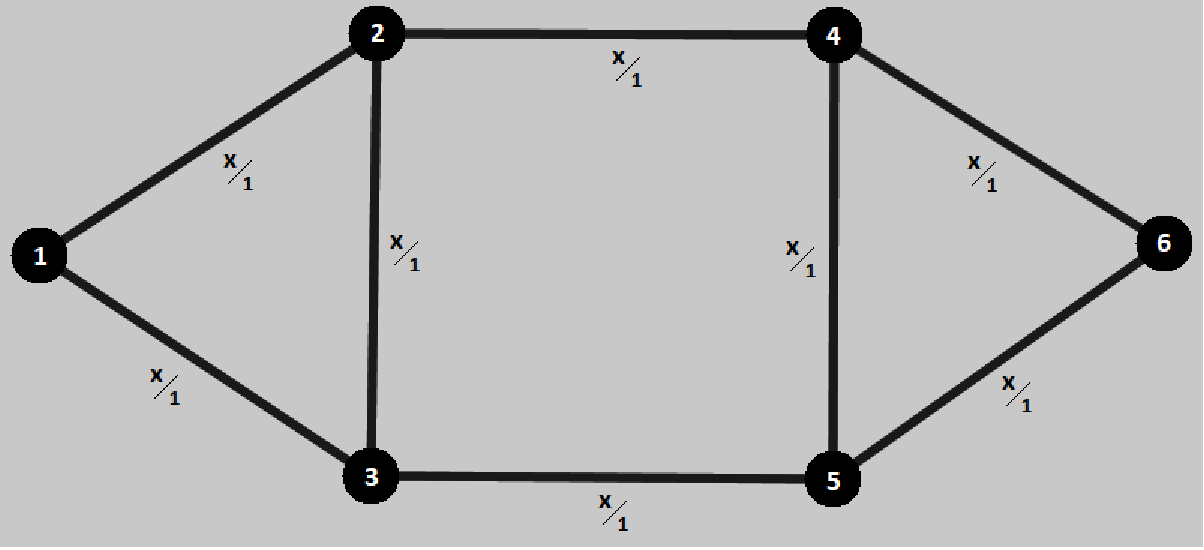
\includegraphics[width=13cm]{sdf/heuristic/transparent_protection/figures/allowed_physical}
\caption{Allowed physical topology. The allowed physical topology is defined by the duct and sites in the field. It is assumed that each duct supports up to 1 bidirectional transmission system and each site supports up to 1 node.}
\label{allowed_physical_protection_ref_low_heuristic_transparent}
\end{figure}

\begin{figure}[H]
\centering
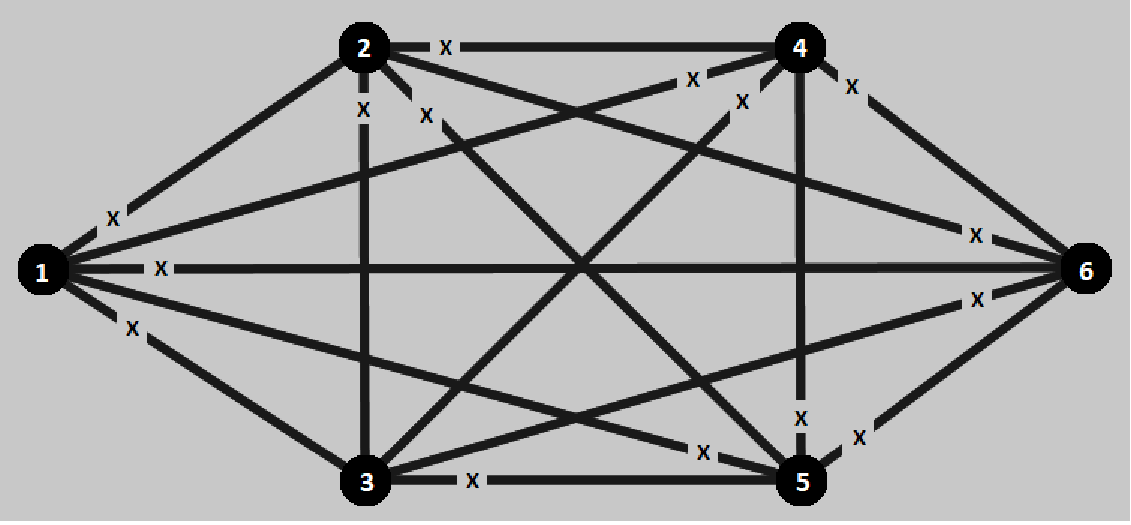
\includegraphics[width=13cm]{sdf/heuristic/transparent_protection/figures/allowed_optical}
\caption{Allowed optical topology. The allowed optical topology is defined by the transport mode (transparent transport mode in this case). It is assumed that each connections between demands supports up to 100 lightpaths.}
\label{allowed_optical_protection_ref_low_heuristic_transparent}
\end{figure}

\begin{figure}[H]
\centering
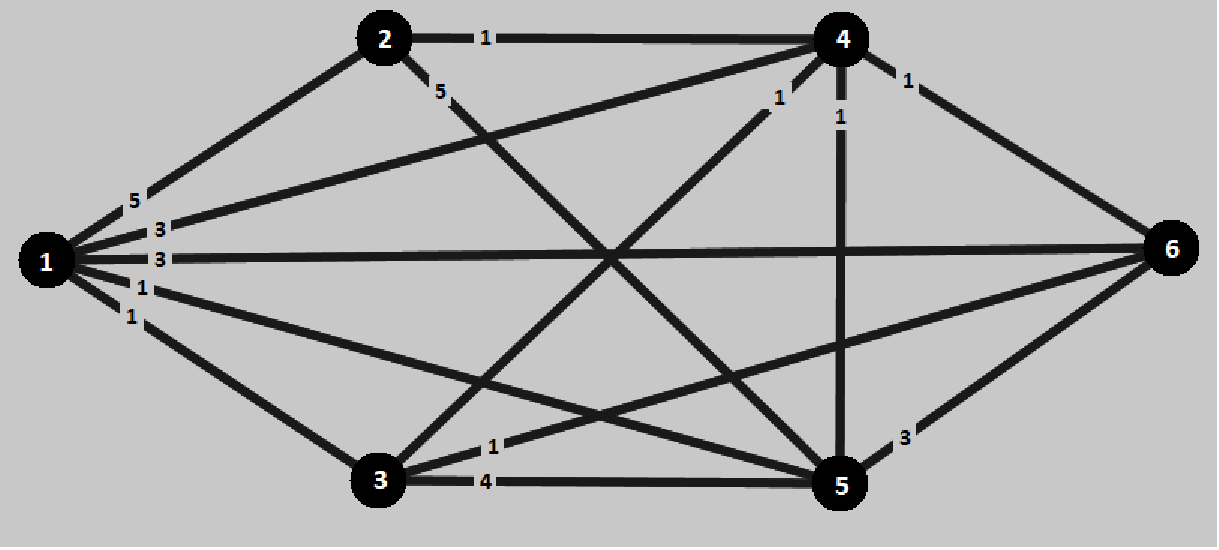
\includegraphics[width=13cm]{sdf/heuristic/transparent_protection/figures/logical_topology_odu0_low}
\caption{ODU0 logical topology defined by the ODU0 traffic matrix.}
\label{logical_ODU0_protection_ref_low_heuristic_transparent}
\end{figure}

\begin{figure}[H]
\centering
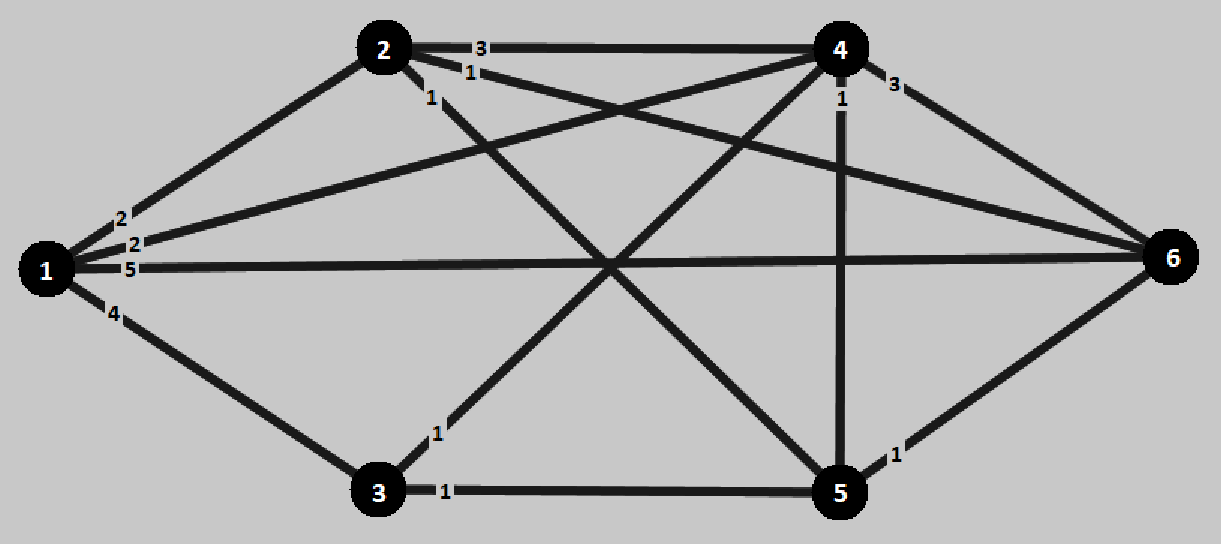
\includegraphics[width=13cm]{sdf/heuristic/transparent_protection/figures/logical_topology_odu1_low}
\caption{ODU1 logical topology defined by the ODU1 traffic matrix.}
\label{logical_ODU1_protection_ref_low_heuristic_transparent}
\end{figure}

\begin{figure}[H]
\centering
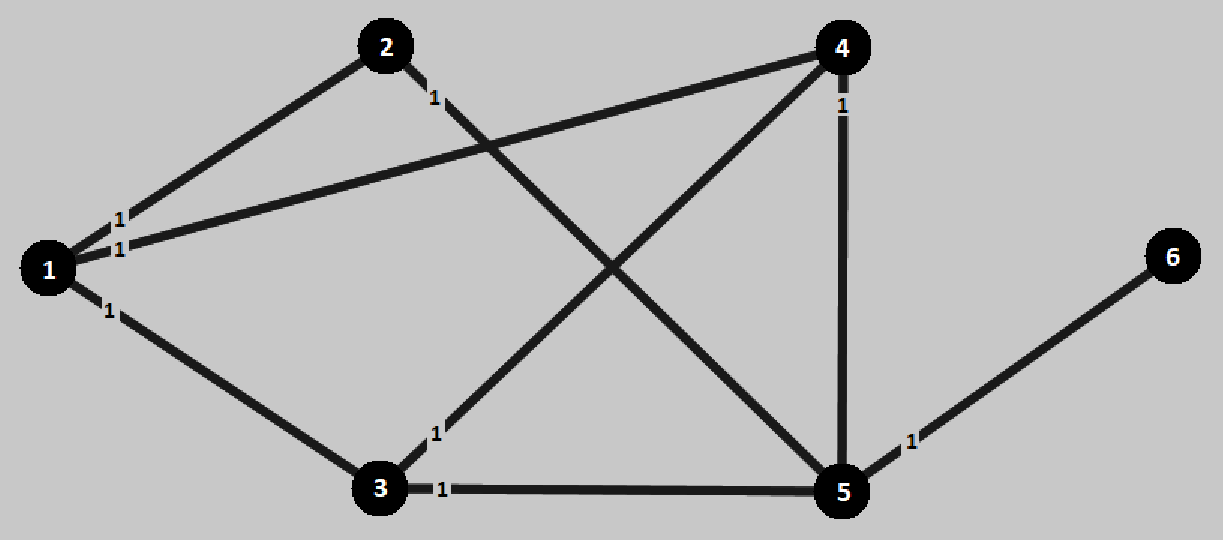
\includegraphics[width=13cm]{sdf/heuristic/transparent_protection/figures/logical_topology_odu2_low}
\caption{ODU2 logical topology defined by the ODU2 traffic matrix.}
\label{logical_ODU2_protection_ref_low_heuristic_transparent}
\end{figure}

\begin{figure}[H]
\centering
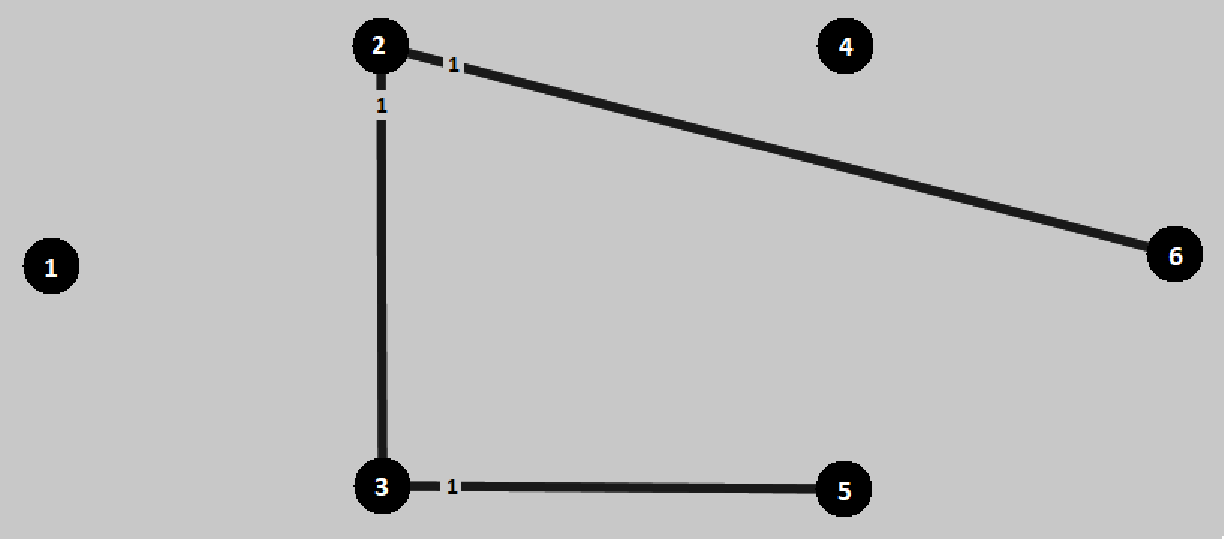
\includegraphics[width=13cm]{sdf/heuristic/transparent_protection/figures/logical_topology_odu3_low}
\caption{ODU3 logical topology defined by the ODU3 traffic matrix.}
\label{logical_ODU3_protection_ref_low_heuristic_transparent}
\end{figure}

\begin{figure}[H]
\centering
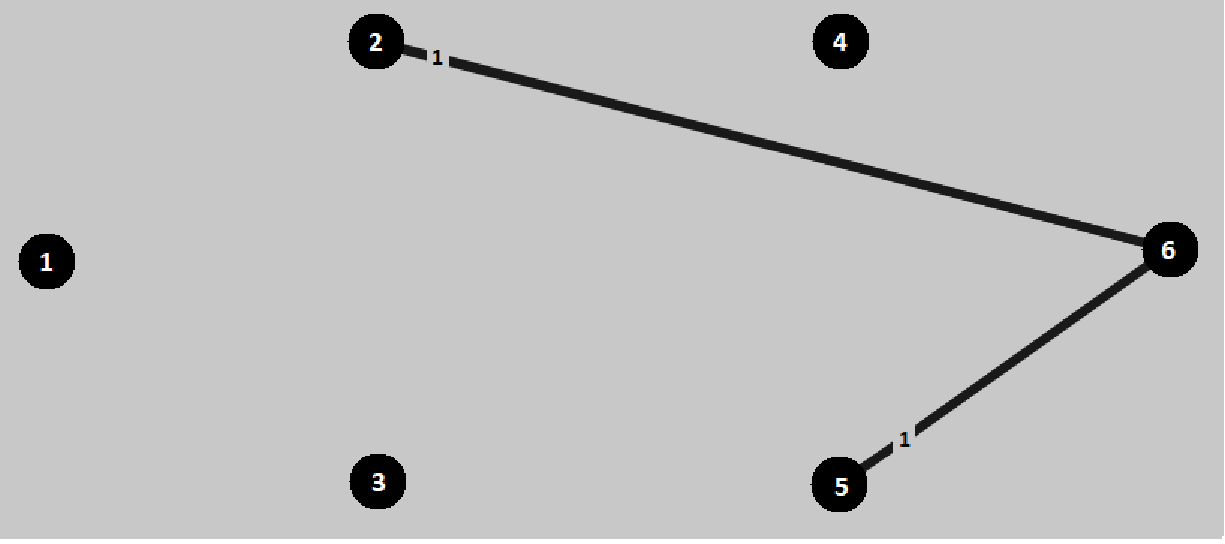
\includegraphics[width=13cm]{sdf/heuristic/transparent_protection/figures/logical_topology_odu4_low}
\caption{ODU4 logical topology defined by the ODU4 traffic matrix.}
\label{logical_ODU4_protection_ref_low_heuristic_transparent}
\end{figure}

\begin{figure}[H]
\centering
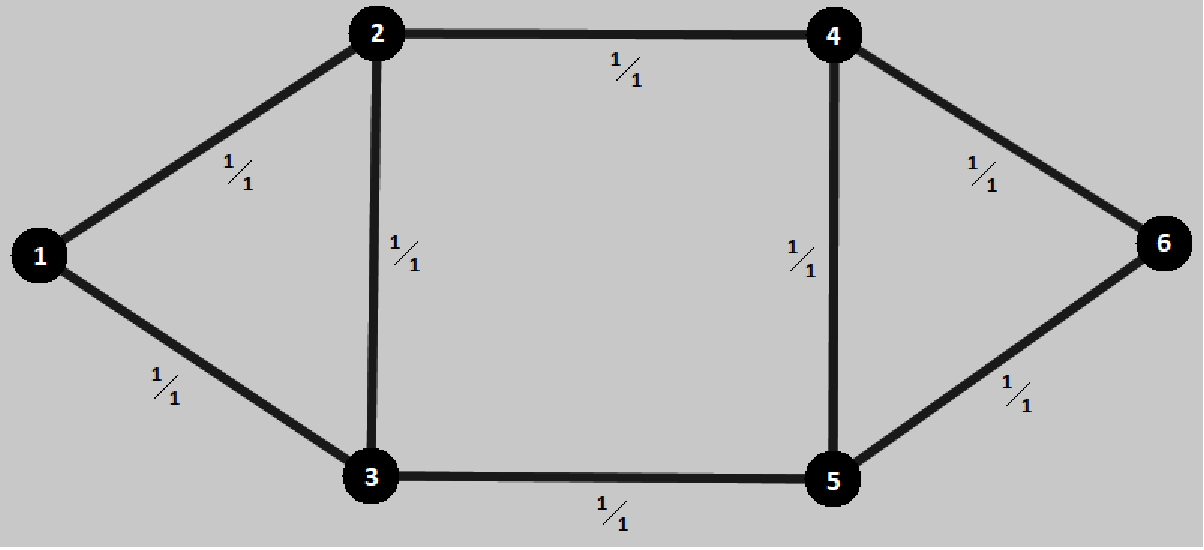
\includegraphics[width=13cm]{sdf/heuristic/transparent_protection/figures/physical_topology}
\caption{Physical topology after dimensioning.}
\label{physical_topology_protection_ref_low_heuristic_transparent}
\end{figure}

Following all the steps mentioned in the \ref{net2plan_guide}, applying the routing and grooming heuristic algorithms in the Net2Plan software and using all the data referring to this scenario, the obtained result for the Vasco's heuristics can be consulted in the following table \ref{scripttransp_protec_ref_low_heuristic}. In table \ref{formulas_transp_heuristic} mentioned in previous model we can see how all the values were calculated. \\

\begin{table}[H]
\centering
\begin{tabular}{|| c | c | c | c | c | c | c ||}
 \hline
 \multicolumn{7}{|| c ||}{CAPEX of the Network} \\
 \hline
 \hline
 \multicolumn{3}{|| c |}{ } & Quantity & Unit Price & Cost & Total \\
 \hline
 \multirow{3}{*}{\makecell{Link \\ Cost}} & \multicolumn{2}{ c |}{OLTs} & 16 & 15 000 \euro & 240 000 \euro & \multirow{3}{*}{136 520 000 \euro} \\ \cline{2-6}
 & \multicolumn{2}{ c |}{100 Gbits/s Transceivers} & 136 & 5 000 \euro/Gbit/s & 68 000 000 \euro & \\ \cline{2-6}
 & \multicolumn{2}{ c |}{Amplifiers} & 70 & 4 000 \euro & 280 000 \euro & \\
 \hline
 \multirow{10}{*}{\makecell{Node \\ Cost}} & \multirow{7}{*}{Electrical} & EXCs & 6 & 10 000 \euro & 60 000 \euro & \multirow{10}{*}{4 347 590 \euro} \\ \cline{3-6}
  & & ODU0 Ports & 60 & 10 \euro/port & 600 \euro & \\ \cline{3-6}
 & & ODU1 Ports & 50 & 15 \euro/port & 750 \euro & \\ \cline{3-6}
 & & ODU2 Ports & 16 & 30 \euro/port & 480 \euro & \\ \cline{3-6}
 & & ODU3 Ports & 6 & 60 \euro/port & 360 \euro & \\ \cline{3-6}
 & & ODU4 Ports & 4 & 100 \euro/port & 400 \euro & \\ \cline{3-6}
 & & Transponders & 34 & 100 000 \euro/port & 3 400 000 \euro & \\ \cline{2-6}
 & \multirow{3}{*}{Optical} & OXCs & 6 & 20 000 \euro & 120 000 \euro & \\ \cline{3-6}
 & & Line Ports & 272 & 2 500 \euro/port & 680 000 \euro & \\ \cline{3-6}
 & & Add Ports & 34 & 2 500 \euro/port & 85 000 \euro & \\
 \hline
 \multicolumn{6}{|| c |}{Total Network Cost} & 140 867 590 \euro \\
\hline
\end{tabular}
\caption{Table with detailed description of CAPEX of Vasco's 2016 results.}
\label{scripttransp_protec_ref_low_heuristic}
\end{table}

\textbf{Medium Traffic Scenario:}\\

In this scenario we have to take into account the traffic calculated in \ref{medium_traffic_scenario}. In a first phase we will show the various existing topologies of the network. The first are the allowed topologies, physical and optical topologies, the second are the logical topology for all ODUs and finally the resulting physical topology.\\

\begin{figure}[H]
\centering
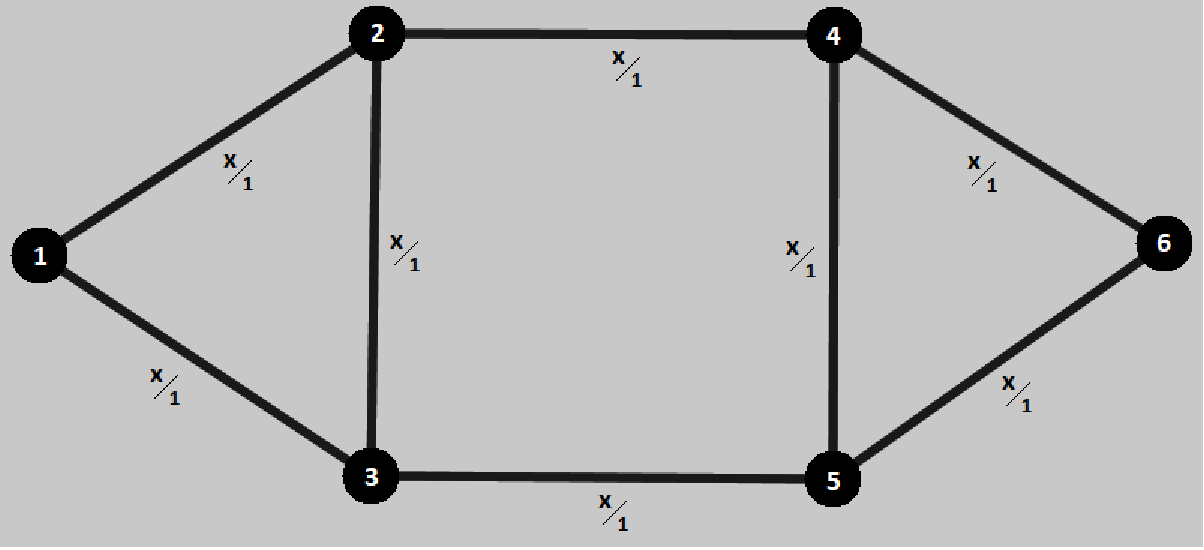
\includegraphics[width=13cm]{sdf/heuristic/transparent_protection/figures/allowed_physical}
\caption{Allowed physical topology. The allowed physical topology is defined by the duct and sites in the field. It is assumed that each duct supports up to 1 bidirectional transmission system and each site supports up to 1 node.}
\label{allowed_physical_protection_ref_medium_heuristic_transparent}
\end{figure}

\begin{figure}[H]
\centering
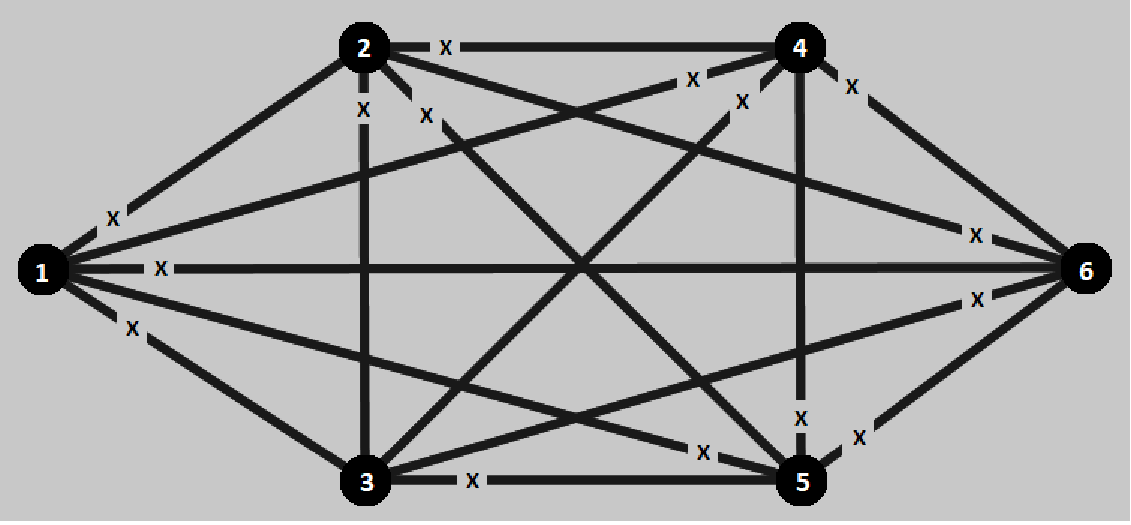
\includegraphics[width=13cm]{sdf/heuristic/transparent_protection/figures/allowed_optical}
\caption{Allowed optical topology. The allowed optical topology is defined by the transport mode (transparent transport mode in this case). It is assumed that each connections between demands supports up to 100 lightpaths.}
\label{allowed_optical_protection_ref_medium_heuristic_transparent}
\end{figure}

\begin{figure}[H]
\centering
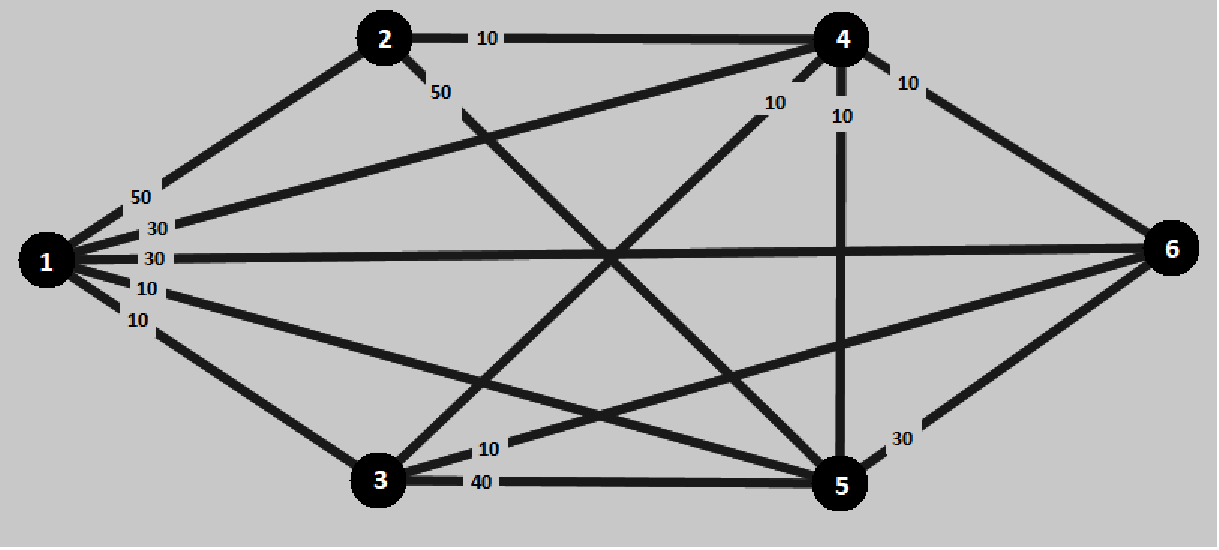
\includegraphics[width=13cm]{sdf/heuristic/transparent_protection/figures/logical_topology_odu0_medium}
\caption{ODU0 logical topology defined by the ODU0 traffic matrix.}
\label{logical_ODU0_protection_ref_medium_heuristic_transparent}
\end{figure}

\begin{figure}[H]
\centering
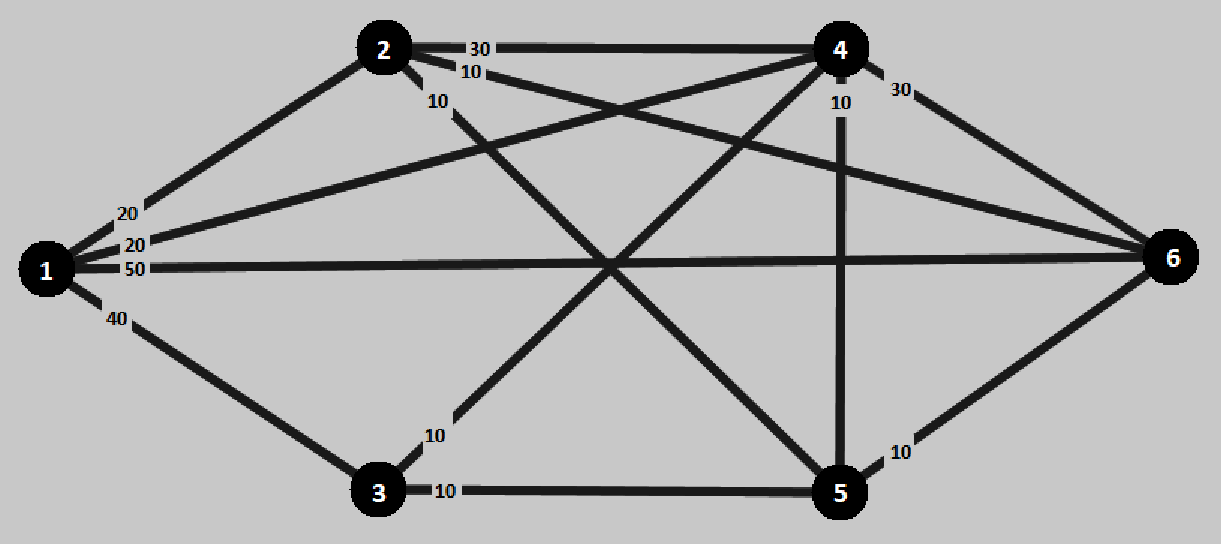
\includegraphics[width=13cm]{sdf/heuristic/transparent_protection/figures/logical_topology_odu1_medium}
\caption{ODU1 logical topology defined by the ODU1 traffic matrix.}
\label{logical_ODU1_protection_ref_medium_heuristic_transparent}
\end{figure}

\begin{figure}[H]
\centering
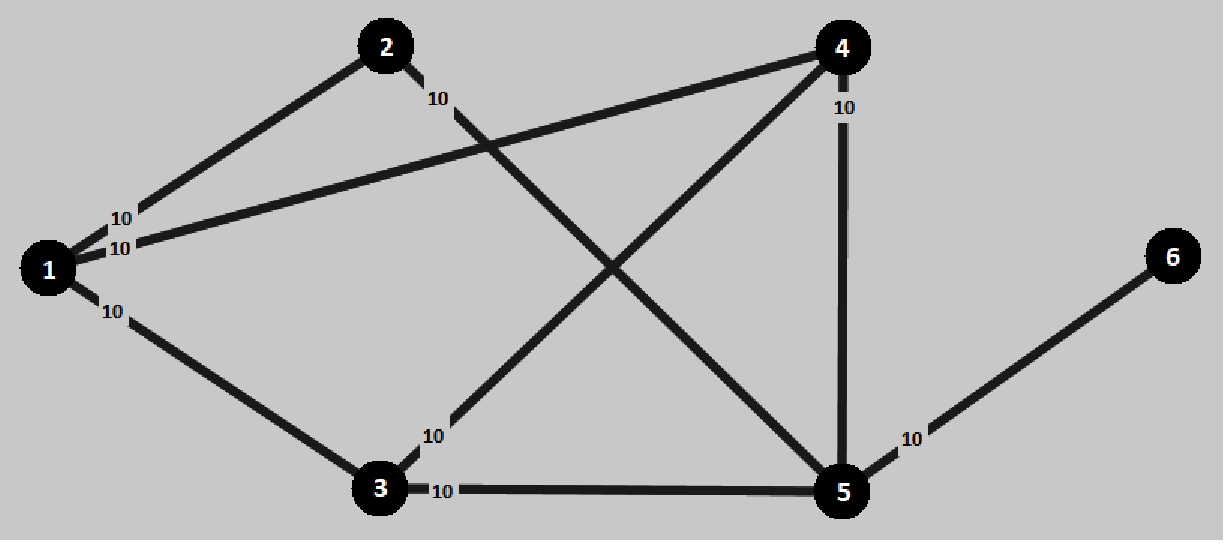
\includegraphics[width=13cm]{sdf/heuristic/transparent_protection/figures/logical_topology_odu2_medium}
\caption{ODU2 logical topology defined by the ODU2 traffic matrix.}
\label{logical_ODU2_protection_ref_medium_heuristic_transparent}
\end{figure}

\begin{figure}[H]
\centering
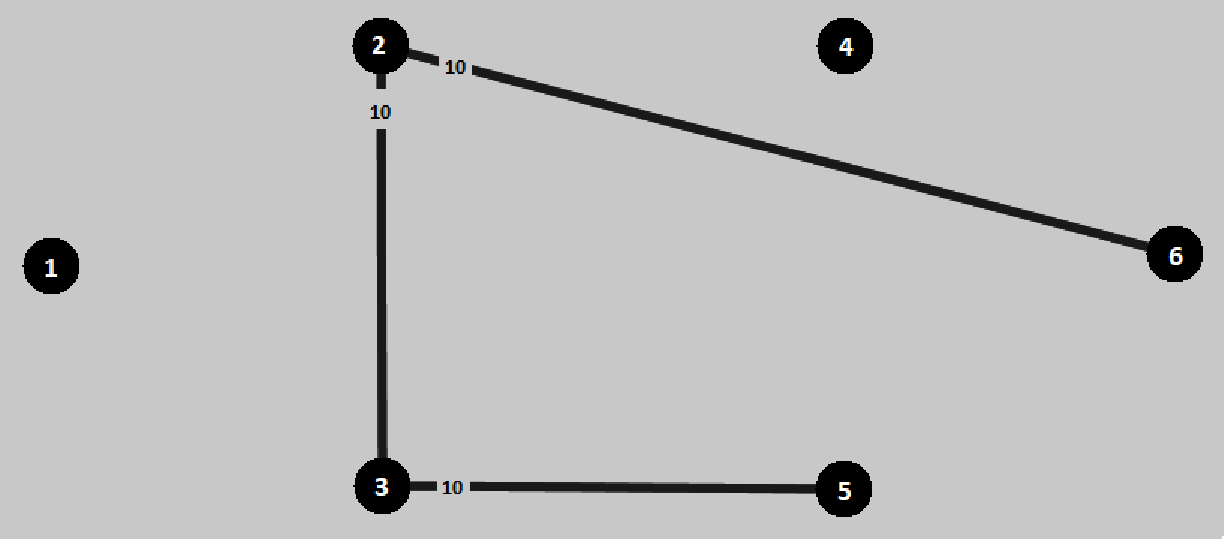
\includegraphics[width=13cm]{sdf/heuristic/transparent_protection/figures/logical_topology_odu3_medium}
\caption{ODU3 logical topology defined by the ODU3 traffic matrix.}
\label{logical_ODU3_protection_ref_medium_heuristic_transparent}
\end{figure}

\begin{figure}[H]
\centering
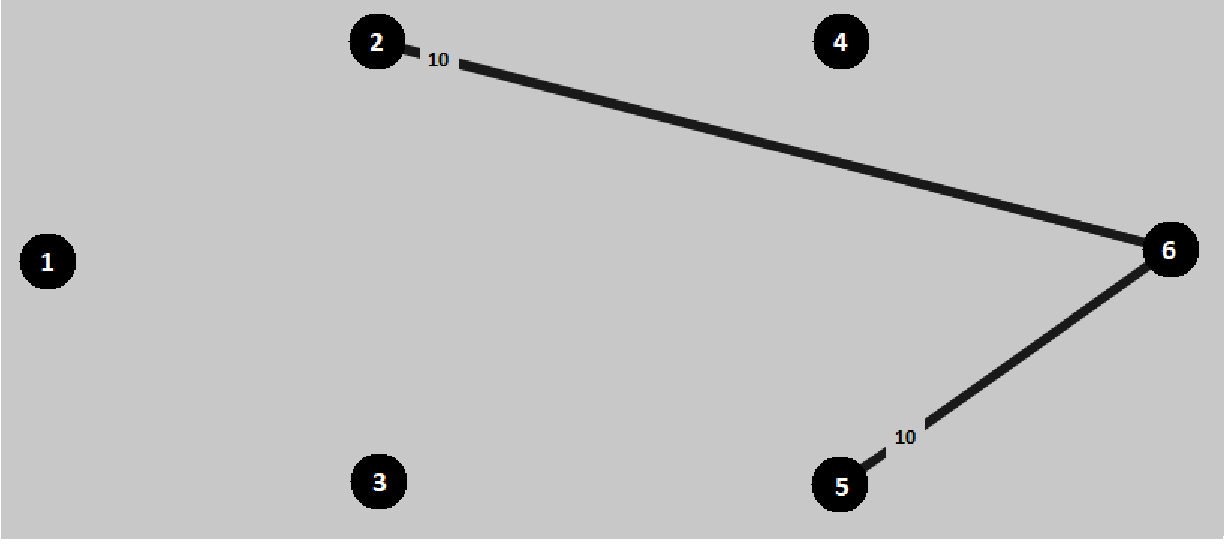
\includegraphics[width=13cm]{sdf/heuristic/transparent_protection/figures/logical_topology_odu4_medium}
\caption{ODU4 logical topology defined by the ODU4 traffic matrix.}
\label{logical_ODU4_protection_ref_medium_heuristic_transparent}
\end{figure}

\begin{figure}[H]
\centering
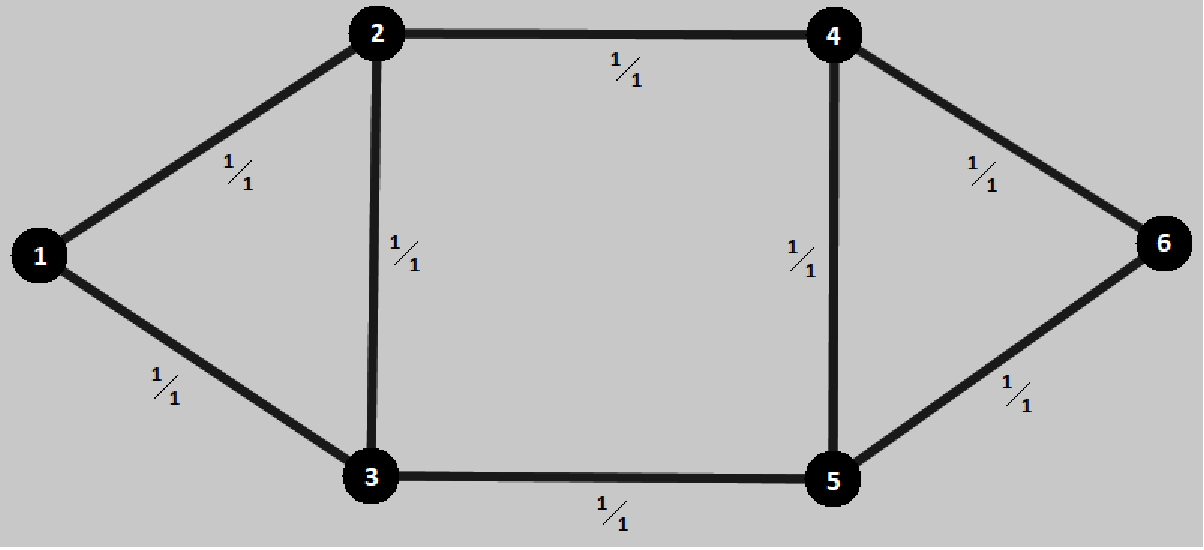
\includegraphics[width=13cm]{sdf/heuristic/transparent_protection/figures/physical_topology}
\caption{Physical topology after dimensioning.}
\label{physical_topology_protection_ref_medium_heuristic_transparent}
\end{figure}

Following all the steps mentioned in the \ref{net2plan_guide}, applying the routing and grooming heuristic algorithms in the Net2Plan software and using all the data referring to this scenario, the obtained result for the Vasco's heuristics can be consulted in the following table \ref{scripttransp_protec_ref_medium_heuristic}. In table \ref{formulas_transp_heuristic} mentioned in previous model we can see how all the values were calculated. \\

\begin{table}[H]
\centering
\begin{tabular}{|| c | c | c | c | c | c | c ||}
 \hline
 \multicolumn{7}{|| c ||}{CAPEX of the Network} \\
 \hline
 \hline
 \multicolumn{3}{|| c |}{ } & Quantity & Unit Price & Cost & Total \\
 \hline
 \multirow{3}{*}{\makecell{Link \\ Cost}} & \multicolumn{2}{ c |}{OLTs} & 16 & 15 000 \euro & 240 000 \euro & \multirow{3}{*}{452 520 000 \euro} \\ \cline{2-6}
 & \multicolumn{2}{ c |}{100 Gbits/s Transceivers} & 452 & 5 000 \euro/Gbit/s & 226 000 000 \euro & \\ \cline{2-6}
 & \multicolumn{2}{ c |}{Amplifiers} & 70 & 4 000 \euro & 280 000 \euro & \\
 \hline
 \multirow{10}{*}{\makecell{Node \\ Cost}} & \multirow{7}{*}{Electrical} & EXCs & 6 & 10 000 \euro & 60 000 \euro & \multirow{10}{*}{14 150 900 \euro} \\ \cline{3-6}
 & & ODU0 Ports & 600 & 10 \euro/port & 6 000 \euro & \\ \cline{3-6}
 & & ODU1 Ports & 500 & 15 \euro/port & 7 500 \euro & \\ \cline{3-6}
 & & ODU2 Ports & 160 & 30 \euro/port & 4 800 \euro & \\ \cline{3-6}
 & & ODU3 Ports & 60 & 60 \euro/port & 3 600 \euro & \\ \cline{3-6}
 & & ODU4 Ports & 40 & 100 \euro/port & 4 000 \euro & \\ \cline{3-6}
 & & Transponders & 114 & 100 000 \euro/port & 11 400 000 \euro & \\ \cline{2-6}
 & \multirow{3}{*}{Optical} & OXCs & 6 & 20 000 \euro & 120 000 \euro & \\ \cline{3-6}
 & & Line Ports & 904 & 2 500 \euro/port & 2 260 000 \euro & \\ \cline{3-6}
 & & Add Ports & 114 & 2 500 \euro/port & 285 000 \euro & \\
 \hline
 \multicolumn{6}{|| c |}{Total Network Cost} & 466 670 900 \euro \\
\hline
\end{tabular}
\caption{Table with detailed description of CAPEX of Vasco's 2016 results.}
\label{scripttransp_protec_ref_medium_heuristic}
\end{table}

\textbf{High Traffic Scenario:}\\

In this scenario we have to take into account the traffic calculated in \ref{high_traffic_scenario}. In a first phase we will show the various existing topologies of the network. The first are the allowed topologies, physical and optical topologies, the second are the logical topology for all ODUs and finally the resulting physical topology.\\

\begin{figure}[H]
\centering
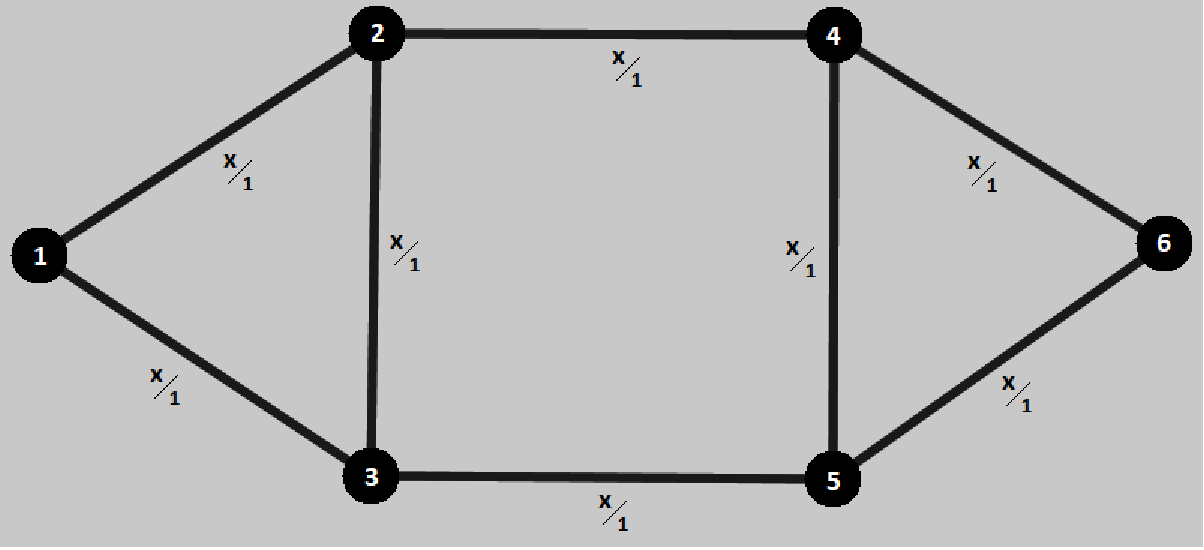
\includegraphics[width=13cm]{sdf/heuristic/transparent_protection/figures/allowed_physical}
\caption{Allowed physical topology. The allowed physical topology is defined by the duct and sites in the field. It is assumed that each duct supports up to 1 bidirectional transmission system and each site supports up to 1 node.}
\label{allowed_physical_protection_ref_high_heuristic_transparent}
\end{figure}

\begin{figure}[H]
\centering
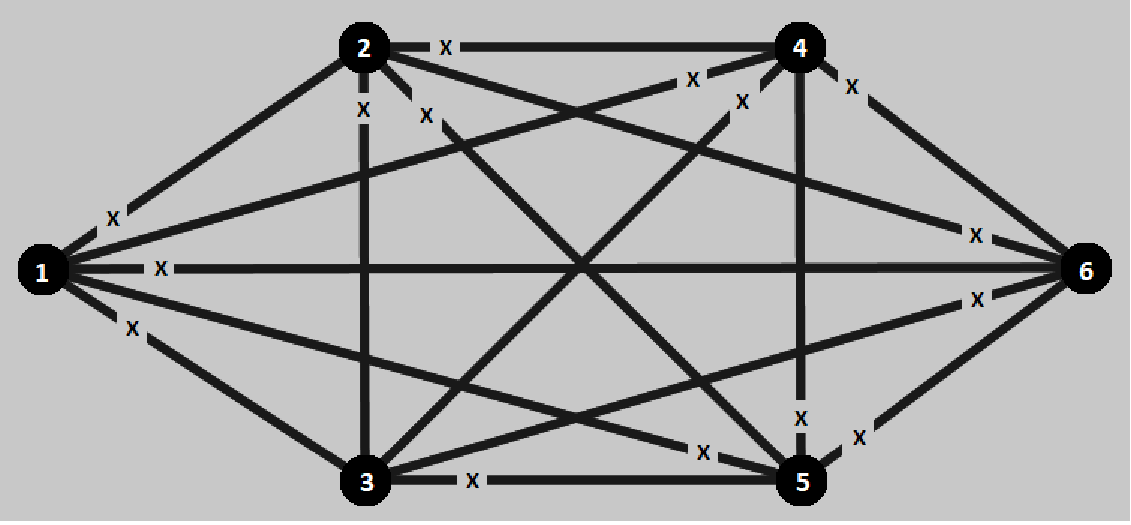
\includegraphics[width=13cm]{sdf/heuristic/transparent_protection/figures/allowed_optical}
\caption{Allowed optical topology. The allowed optical topology is defined by the transport mode (transparent transport mode in this case). It is assumed that each connections between demands supports up to 100 lightpaths.}
\label{allowed_optical_protection_ref_high_heuristic_transparent}
\end{figure}

\begin{figure}[H]
\centering
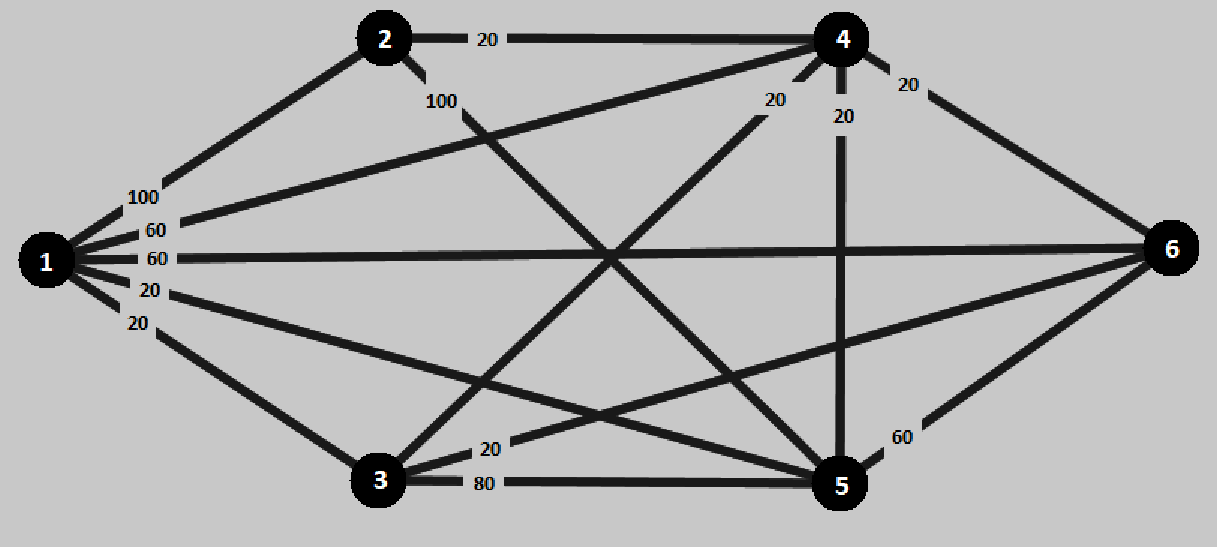
\includegraphics[width=13cm]{sdf/heuristic/transparent_protection/figures/logical_topology_odu0_high}
\caption{ODU0 logical topology defined by the ODU0 traffic matrix.}
\label{logical_ODU0_protection_ref_high_heuristic_transparent}
\end{figure}

\begin{figure}[H]
\centering
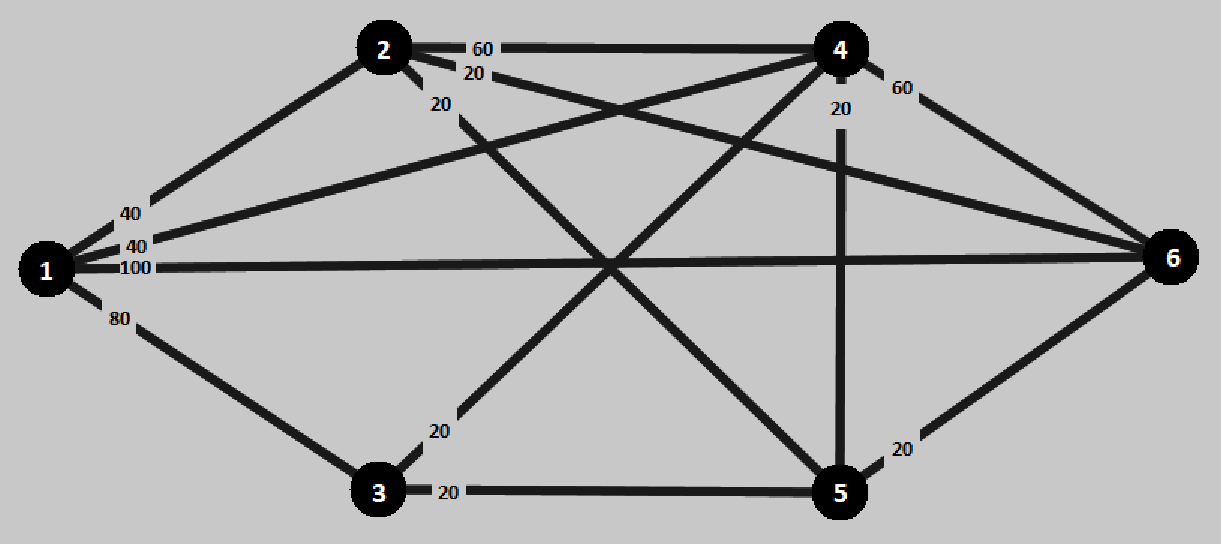
\includegraphics[width=13cm]{sdf/heuristic/transparent_protection/figures/logical_topology_odu1_high}
\caption{ODU1 logical topology defined by the ODU1 traffic matrix.}
\label{logical_ODU1_protection_ref_high_heuristic_transparent}
\end{figure}

\begin{figure}[H]
\centering
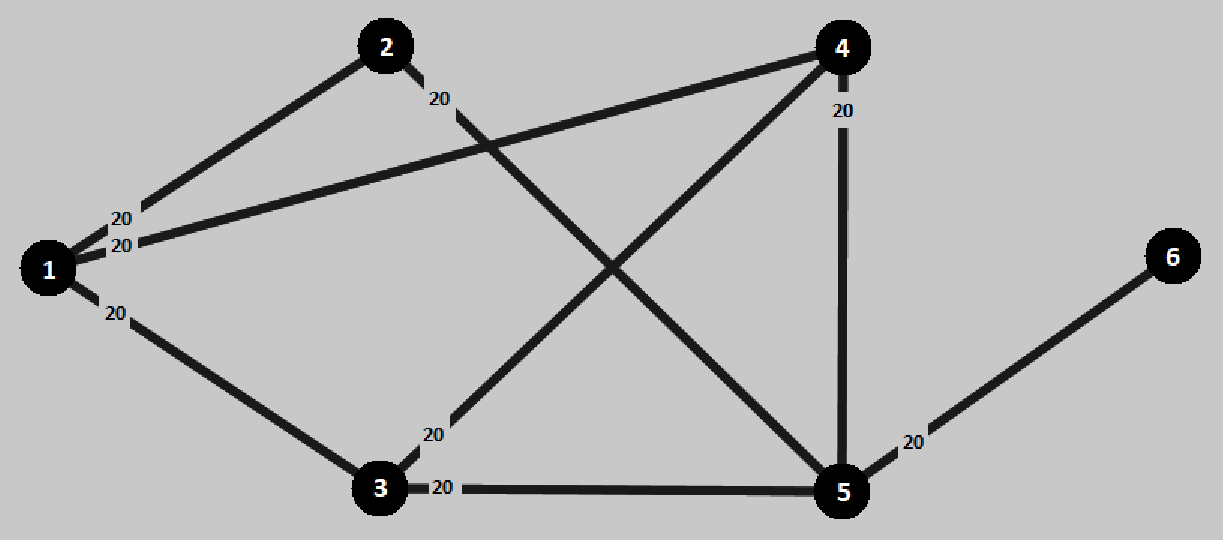
\includegraphics[width=13cm]{sdf/heuristic/transparent_protection/figures/logical_topology_odu2_high}
\caption{ODU2 logical topology defined by the ODU2 traffic matrix.}
\label{logical_ODU2_protection_ref_high_heuristic_transparent}
\end{figure}

\begin{figure}[H]
\centering
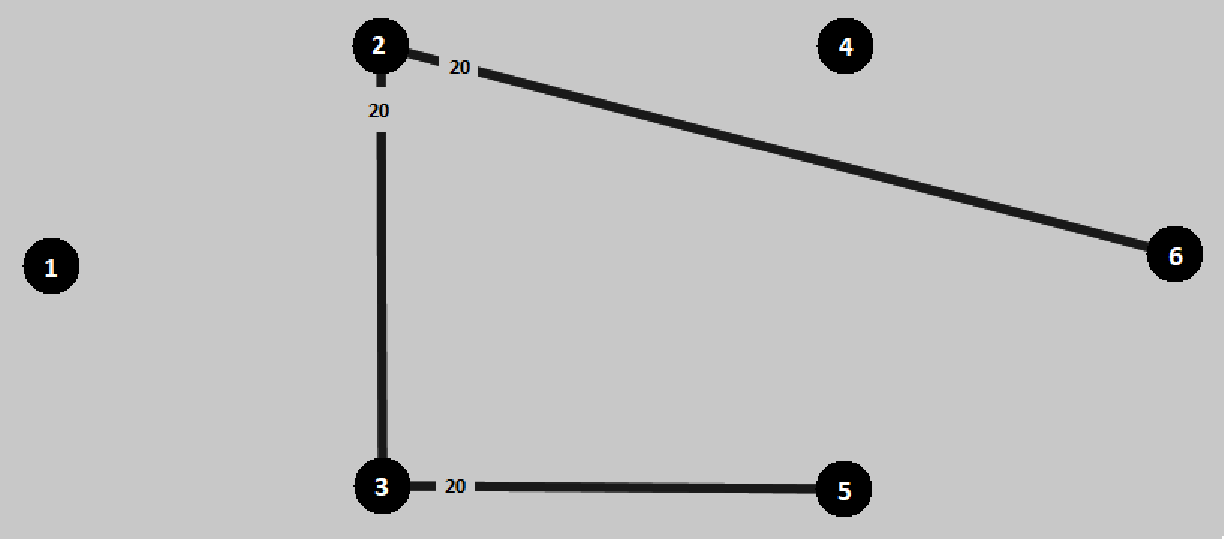
\includegraphics[width=13cm]{sdf/heuristic/transparent_protection/figures/logical_topology_odu3_high}
\caption{ODU3 logical topology defined by the ODU3 traffic matrix.}
\label{logical_ODU3_protection_ref_high_heuristic_transparent}
\end{figure}

\begin{figure}[H]
\centering
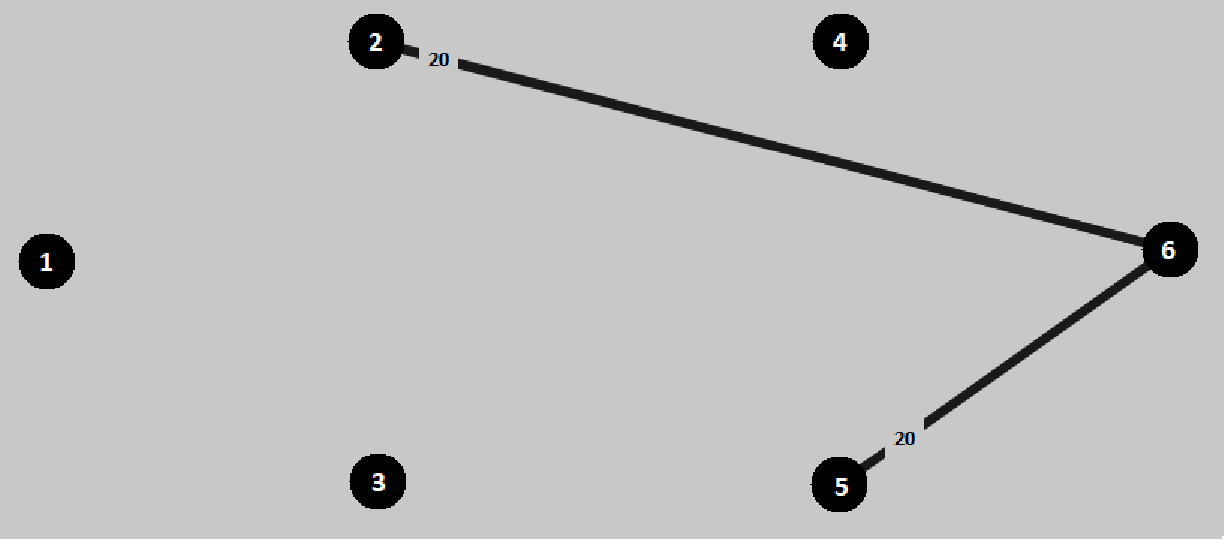
\includegraphics[width=13cm]{sdf/heuristic/transparent_protection/figures/logical_topology_odu4_high}
\caption{ODU4 logical topology defined by the ODU4 traffic matrix.}
\label{logical_ODU4_protection_ref_high_heuristic_transparent}
\end{figure}

\begin{figure}[H]
\centering
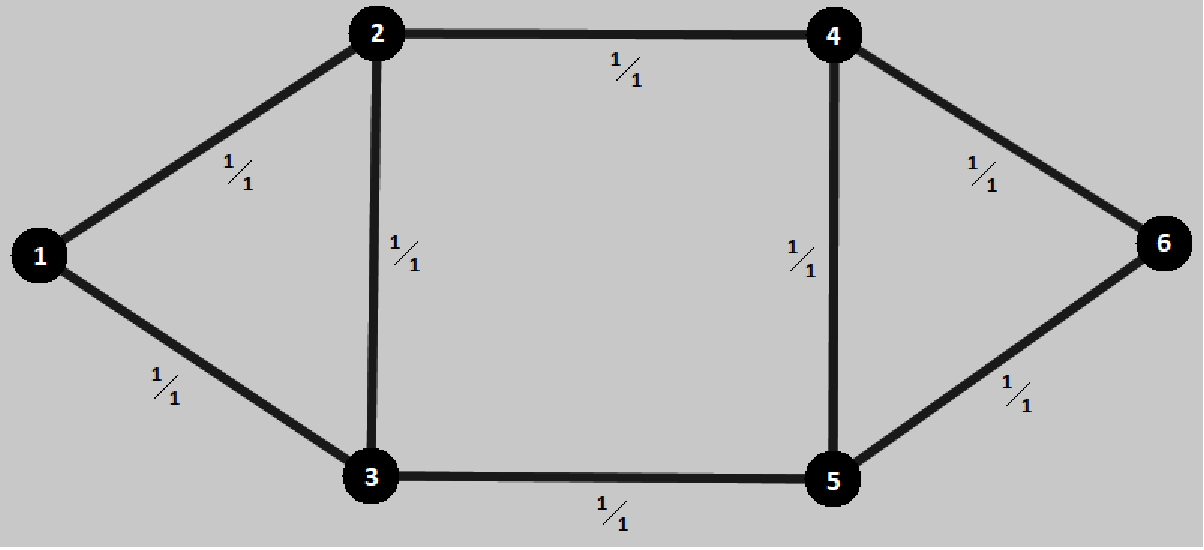
\includegraphics[width=13cm]{sdf/heuristic/transparent_protection/figures/physical_topology}
\caption{Physical topology after dimensioning.}
\label{physical_topology_protection_ref_high_heuristic_transparent}
\end{figure}

Following all the steps mentioned in the \ref{net2plan_guide}, applying the routing and grooming heuristic algorithms in the Net2Plan software and using all the data referring to this scenario, the obtained result for the Vasco's heuristics can be consulted in the following table \ref{scripttransp_protec_ref_high_heuristic}. In table \ref{formulas_transp_heuristic} mentioned in previous model we can see how all the values were calculated. \\

\begin{table}[H]
\centering
\begin{tabular}{|| c | c | c | c | c | c | c ||}
 \hline
 \multicolumn{7}{|| c ||}{CAPEX of the Network} \\
 \hline
 \hline
 \multicolumn{3}{|| c |}{ } & Quantity & Unit Price & Cost & Total \\
 \hline
 \multirow{3}{*}{\makecell{Link \\ Cost}} & \multicolumn{2}{ c |}{OLTs} & 16 & 15 000 \euro & 240 000 \euro & \multirow{3}{*}{848 520 000 \euro} \\ \cline{2-6}
 & \multicolumn{2}{ c |}{100 Gbits/s Transceivers} & 848 & 5 000 \euro/Gbit/s & 424 000 000 \euro & \\ \cline{2-6}
 & \multicolumn{2}{ c |}{Amplifiers} & 70 & 4 000 \euro & 280 000 \euro & \\
 \hline
 \multirow{10}{*}{\makecell{Node \\ Cost}} & \multirow{7}{*}{Electrical} & EXCs & 6 & 10 000 \euro & 60 000 \euro & \multirow{10}{*}{26 406 800 \euro} \\ \cline{3-6}
  & & ODU0 Ports & 1 200 & 10 \euro/port & 12 000 \euro & \\ \cline{3-6}
 & & ODU1 Ports & 1 000 & 15 \euro/port & 15 000 \euro & \\ \cline{3-6}
 & & ODU2 Ports & 320 & 30 \euro/port & 9 600 \euro & \\ \cline{3-6}
 & & ODU3 Ports & 120 & 60 \euro/port & 7 200 \euro & \\ \cline{3-6}
 & & ODU4 Ports & 80 & 100 \euro/port & 8 000 \euro & \\ \cline{3-6}
 & & Transponders & 214 & 100 000 \euro/port & 21 400 000 \euro & \\ \cline{2-6}
 & \multirow{3}{*}{Optical} & OXCs & 6 & 20 000 \euro & 120 000 \euro & \\ \cline{3-6}
 & & Line Ports & 1 696 & 2 500 \euro/port & 4 240 000 \euro & \\ \cline{3-6}
 & & Add Ports & 214 & 2 500 \euro/port & 535 000 \euro & \\
 \hline
 \multicolumn{6}{|| c |}{Total Network Cost} & 874 926 800 \euro \\
\hline
\end{tabular}
\caption{Table with detailed description of CAPEX of Vasco's 2016 results.}
\label{scripttransp_protec_ref_high_heuristic}
\end{table}

\vspace{13pt}

\subsubsection{Conclusions}

Once we have obtained the results for all the scenarios for transparent without survivability and transparent with 1+1 protection we will now draw some conclusions about these results. For a better analysis of the results will be created the table \ref{table_comparative_transparent_protec_heuristic} with the number of line ports, tributary ports and transceivers because they are important values for the cost of CAPEX, the cost of links, the cost of nodes and finally the cost of CAPEX.\\

\begin{table}[H]
\centering
\begin{tabular}{| c | c | c | c |}
 \hline
 & Low Traffic & Medium Traffic & High Traffic \\
 \hline\hline
 \makecell{CAPEX \\ without survivability} & 56 447 590 \euro & 181 250 900 \euro & 338 256 800 \euro \\ \hline
 \makecell{CAPEX/Gbit/s \\ without survivability} & 112 895 \euro/Gbit/s & 36 250 \euro/Gbit/s & 33 825 \euro/Gbit/s \\ \hline
 Traffic (Gbit/s) & 500 & 5 000 & 10 000 \\ \hline
 Bidirectional Links used & 8 & 8 & 8 \\ \hline
 Number of Add ports & 34 & 114 & 214 \\ \hline
 Number of Line ports & 272 & 904 & 1 696 \\ \hline
 Number of Tributary ports & 136 & 1 360 & 2 720 \\ \hline
 Number of Transceivers & 272 & 904 & 1 696 \\ \hline
 Link Cost & 136 520 000 \euro & 452 520 000 \euro & 848 520 000 \euro \\ \hline
 Node Cost & 4 347 590 \euro & 14 150 900 \euro & 26 406 800 \euro \\ \hline
 CAPEX & \textbf{140 867 590 \euro} & \textbf{466 670 900 \euro} & \textbf{874 926 800 \euro} \\ \hline
 CAPEX/Gbit/s & \textbf{281 735 \euro/Gbit/s} & \textbf{93 334 \euro/Gbit/s} & \textbf{87 492 \euro/Gbit/s} \\ \hline
\end{tabular}
\caption{Table with different value of CAPEX for this case.}
\label{table_comparative_transp_protec_heuristic}
\end{table}

\noindent
Looking at the previous table we can make some comparisons between the transparent with 1+1 protection scenario:

\begin{itemize}
  \item Comparing the low traffic with the others we can see that despite having an increase of factor ten (medium traffic) and factor twenty (high traffic), the same increase does not occur in the final cost (it is lower);
  \subitem This happens because the number of the transceivers is lower than expected which leads by carrying the traffic with less network components and, consequently, the network CAPEX is lower;
  \item Comparing the medium traffic with the high traffic we can see that the increase of the factor is double and in the final cost this factor is very close but still inferior;
  \subitem This happens because the number of the transceivers is also lower but very close to the expected;
  \item Comparing the CAPEX cost per bit we can see that in the low traffic the cost is higher than the medium and high traffic, which in these two cases the value is similar, but still inferior in the higher traffic;
  \subitem This happens because the lower the traffic, the higher CAPEX/bit will be. We can see that in medium and high traffic the results tend to be one closer and lower value.
\end{itemize}

\noindent
We can also make some comparisons between the transparent without survivability and transparent with 1+1 protection scenarios:

\begin{itemize}
  \item We can see that in the transparent with 1+1 protection the CAPEX cost for all the three traffic is more than the double;
    \subitem This happens because in the transparent with 1+1 protection there is a need of having a primary and a backup path, in case of a network failure, and the backup path is typically longer;
  \item Comparing the CAPEX cost per bit we can see that has a similar case in both of the two scenarios. In the low traffic the cost is higher than the medium and high traffic, which in these two cases the value is similar;
  \subitem This happens because the lower the traffic, the higher CAPEX/bit will be. We can see that in medium and high traffic the results tend to be one closer and lower value.
\end{itemize}

\vspace{13pt}
\subsubsection{Opens Issues}

The creation of this model for any scenario, started with some considerations and some open issues being:

\begin{itemize}
  \item Allow blocking.
  \subitem The presented model assume that the solution is possible or impossible, does not support a partial solution where some demands are not routed (are blocked);
  \item Allow multiple transmission system.
  \subitem The presented model for each link only supports one transmission system.
\end{itemize} 